%%%%%%%%%%%%%%%%%%%%%%%%%%%%%%%%%%%%%%%%%%%%%%%%%%%%%%%%%%%%%%%%%%%%%%
%%	Name: "Signal analysis template"
%%	File name: signalanalysis_template_main
%%	Version: 1.5
%%
%%	Compiler: XeLaTeX
%%
%%%%%%%%%%%%%%%%%%%%%%%%%%%%%%%%%%%%%%%%%%%%%%%%%%%%%%%%%%%%%%%%%%%%%%

\documentclass[conference,compsoc,onecolumn]{IEEEtran}

% *** LANGUAGE UTILITY PACKAGES ***
\usepackage[utf8]{inputenc} % Required for including letters with accents
\usepackage[spanish]{babel}
\usepackage{amsmath, amsthm, amssymb}
\usepackage{array}




% *** USED PACKAGES ***
% *** MISC UTILITY PACKAGES ***
\usepackage{comment}			% Agregar comentarios
\usepackage{lipsum}				% Inserts dummy text
\usepackage{blindtext}
\usepackage{listings}					% Coding
\usepackage{verbatim}				% Verbatim
\usepackage[final]{pdfpages}
\usepackage{booktabs,dcolumn}
\usepackage{pdflscape}
\usepackage{afterpage}
\usepackage{parskip}
\usepackage[utf8]{inputenc}
%\setlist[itemize]{noitemsep, nolistsep}
\usepackage[bookmarks=false]{hyperref}
\usepackage{tcolorbox}									% Coloured boxes, for LATEX examples and theorems, etc
\usepackage{color}
\usepackage{xcolor} % Required for specifying colors by name									% Color packages foreground and back­ground color man­age­men
% *** CITATION PACKAGES ***
\usepackage{cite}
% *** GRAPHICS RELATED PACKAGES ***
\usepackage[utf8]{inputenc}
\usepackage{graphicx}
\usepackage{subfig}
\usepackage{caption}
\usepackage{subcaption}
\usepackage{pgfplots}
\usepackage{tikz}
\usetikzlibrary{shapes,arrows}
\usetikzlibrary{decorations.pathmorphing} % noisy shapes
\usetikzlibrary{fit}					% fitting shapes to coordinates
\usetikzlibrary{backgrounds}	% drawing the background after the foreground
\pgfplotsset{compat=1.13}
% *** MATH PACKAGES ***
\usepackage{amsmath}
\usepackage{mathtools}
\usepackage{amssymb}
\usepackage{amsfonts}
\usepackage{expl3}
\usepackage{bm}

% *** SPECIALIZED LIST PACKAGES ***
\usepackage{algorithmic}
\usepackage{listings}					% Coding
\usepackage[framed,numbered,autolinebreaks,useliterate]{mcode}
% *** ALIGNMENT PACKAGES ***
\usepackage{array}
% *** SUBFIGURE PACKAGES ***
%\ifCLASSOPTIONcompsoc
%\usepackage[caption=false,font=normalsize,labelfont=sf,textfont=sf]{subfig}
%\else
%\usepackage[caption=false,font=footnotesize]{subfig}
%\fi
% *** FLOAT PACKAGES ***
\usepackage{fixltx2e}
\usepackage{stfloats}
%\fnbelowfloat
%\usepackage{dblfloatfix}
% *** PDF, URL AND HYPERLINK PACKAGES ***
\usepackage{url}
\usepackage{everypage}


\usepackage{multirow} % In order to be able to insert rows spanning multiple lines
\usepackage{verbatim}
\usepackage[all]{xy}
\usepackage{listings}
\usepackage{subfigure}
\usepackage{multibib}
\usepackage{setspace} 
\usepackage{algorithm}			    	  % To insert nice algorithms

% *** CARPETA DONDE SE GUARDARAN LAS IMAGENES ***
\graphicspath{{figures/}}
% *** NUEVOS COMANDOS Y CONFIGURACIONES VARIAS ***
\interdisplaylinepenalty=2500
\newcommand{\Lpagenumber}{\ifdim\textwidth=\linewidth\else\bgroup
	\dimendef\margin=0
	\ifodd\value{page}\margin=\oddsidemargin
	\else\margin=\evensidemargin
	\fi
	\raisebox{\dimexpr -\topmargin-\headheight-\headsep-0.5\linewidth}[0pt][0pt]{%
		\rlap{\hspace{\dimexpr \margin+\textheight+\footskip}%
			\llap{\rotatebox{90}{\thepage}}}}%
	\egroup\fi}

\AddEverypageHook{\Lpagenumber}%

\newcommand{\newtxt}[1]{\textcolor{black}{#1}}
\renewcommand\IEEEkeywordsname{Palabras cláve:}
\newcommand{\mx}[1]{\mathbf{\bm{#1}}} % Matrix command
\newcommand{\vc}[1]{\mathbf{\bm{#1}}} % Vector command

%% Separación de palabras
\hyphenation{op-tical net-works semi-conduc-tor HHMMSS}
\setlength{\parindent}{1.5em}
\definecolor{negro}{RGB}{255,255,255}
\begin{document}

% *** TITLES AND NAMES ***
% title of the document
\title{Plataforma de seguimiento de datos COVID-19 para Colombia}
% author names and affiliations



\author{\IEEEauthorblockN{Johan~Sebastian~Miranda~Gualdron}
\IEEEauthorblockA{Escuela de Ciencias Exactas\\
U. Sergio Arboleda-Bogotá, Colombia\\
johan.miranda@correo.usa.edu.co}
\and
\IEEEauthorblockN{Luis~Alejandro~Vejarano~Gutierrez}
\IEEEauthorblockA{Escuela de Ciencias Exactas\\
U. Sergio Arboleda-Bogotá, Colombia\\
luis.vejarano01@correo.usa.edu.co}}
% *** MAKE TITLE ***
\maketitle
\IEEEoverridecommandlockouts
\IEEEpeerreviewmaketitle

\begin{abstract}
En el presente informe se explica como extraer datos actualizados referentes al COVID-19 en Colombia, y guardarlos en una base de datos local. Dichos datos son analizados y representados en forma de gráficas y diagramas de una forma selectiva para su mayor entendimiento.
\end{abstract}


\begin{IEEEkeywords}
 Gráficas, bases de datos, python, COVID-19, diagramas, código, análisis de datos .
\end{IEEEkeywords}


\section{Marco teórico}
\label{sec:introduction}

\begin{itemize}
\item\textbf{Python}:Es un lenguaje de programación interpretado,dinámico y multiplataforma, con un código basado en un concepto de eficiencia para ser leído y entendido. \\
Se implementan un código:
    \begin{itemize}
        {\item \textbf{Pandas}: Convierte el archivo JSON en un dataframe.
        \item\textbf{Socrata}: Realiza la petición a la pagina web(HTTP), mediante un token  
      \item\textbf{Graficas}:Representaciones en forma de tortas, barras, de los datos extraídos en la pagina web, implementadas con guía de la pagina web\cite{Graficas} 
      \item\textbf{Librerias}: Es un conjunto de implementaciones funcionales, codificadas en un lenguaje de programación, que ofrece una interfaz bien definida para la funcionalidad que se invoca}
    \end{itemize}


\item\textbf{Tipos de Datos}:
 \begin{itemize}
   {\item\textbf{JSON}:Son archivos usados para almacenar estructuras de datos simples con un registro de texto legible para el usuario, ya sean listas, bases de datos. 
   \item\textbf{Dataframe}: Es una estructura de datos tabulares que permite el manejo de un gran flujo de datos, de una manera mas sencilla.
   \item\textbf{Primitivos}: Son tipos de datos bases en un lenguaje de programación, generalmente están dados por enteros, decimales, y booleanos(verdadero o falso).
   }
   
\end{itemize}
\end{itemize}


\clearpage
\section{Procedimiento}
\subsection{Procedimiento-1 entrega}\label{sec:en1}

\label{sec:procedimiento}
En esta primera entrega, se realizo un código básico donde se utilizaron funciones y comandos para realizar gráficas, tomando como guía los datos actuales sobre los casos de COVID-19 en Colombia.

En la Listing \ref{import} se presentan los import's necesarios para poder realizar la extracción de datos, graficarlos, y poder manejar el tiempo actual para poder imprimirlo en las graficas. 

\lstinputlisting[language=Python, firstline=1, lastline=14, caption=Se importan las librerias, captionpos=b, label=import]{ArchivosM/main.py}

En el Listing \ref{http} se hace uso de Socrata para poder acceder a los datos abiertos de Colombia con un token único el cual se obtuvo al momento de registrarse. Esto se evidencia en la linea 4, donde se invoca Socrata, con el url de la pagina y el token ya mencionado. 
\lstinputlisting[language=Python, firstline=16, lastline=26, caption=Código acceso a datos abiertos-Código respeusta HTTP en pandas Dataframe, captionpos=b, label=http]{ArchivosM/main.py}

Al tener debidamente capturados los datos, los cuales fueron obtenidos mediante una respuesta HTTP, y se realizo una conversión a Pandas Dataframe(Linea 7-11, Listing \ref{http}), para poder realizar consultas mediante el metodo get y su respectivo token. Se procede a realizar el manejo de datos y obtener los debidos graficos.

El código se subdivide en pequeñas secciones para poder identificar rápidamente como se manejo la información y como se genero su respectivo gráfico. Inicialmente se tratan los datos por genero; fue necesario arreglar un error traído de la Base de datos, el cual es el manejo de minúsculas y mayúsculas al momento de realizar la búsqueda de datos, con lo cual, se realiza el código de las lineas 8-16 del Listing \ref{gen} para poder solucionar esto.

\lstinputlisting[language=Python, firstline=29, lastline=54, caption=Código arreglo error mayúsculas y minúsculas-Código gráfica torta Casos por Genero, captionpos=b, label=gen]{ArchivosM/main.py}


De las lineas 20-26 del Listing \ref{gen} se codifica el algoritmo para poder generar la gráfica de Torta de los casos por genero.

Posteriormente se procede a clasificar los casos por ciudades principales(Lineas 1-8; Listing \ref{ciu}), y generar su respectivo gráfico de torta para representar dicha información obtenida de la base de datos en Internet(Lineas 11-19; Listing \ref{ciu}).


\lstinputlisting[language=Python, firstline=56, lastline=74, caption=Código lasificacion de datos por ciudades-Código gráfica torta Casos por Ciudad, captionpos=b, label=ciu]{ArchivosM/main.py}

Otros de los datos registrados en la base de datos, los cuales pueden ser manejados y clasificados son las edades por segmentos, siendo niños de 0-12 años, adolescente de 13-18, jóvenes de 19-26, adulto de 26-59, y ancianos a +60 años. Siguiendo esto se procede a realizar su gráfica expuesta en el código  Listing \ref{edad}.



\lstinputlisting[language=Python, firstline=78, lastline=103, caption=Código clasificación de datos por edades-Código gráfica barras Casos por Edades, captionpos=b, label=edad]{ArchivosM/main.py}

Para finalizar el manejo de datos, se procede a codificar la gráfica del Estado de casos confirmados de COVID-19. Al igual que en anteriores menciones, se debe tratar el problema de las mayúsculas y minúsculas provenientes de la base de datos(Lineas 1-3; Listing  \ref{esta}). 

\lstinputlisting[language=Python, firstline=106, lastline=135, caption=Código clasificación de datos por Estado de los casos-Código gráfica barras Estado de casos, captionpos=b, label=esta]{ArchivosM/main.py}


De las lineas 6-18 en el Listing \ref{esta} se realiza la respectiva clasificación de los datos por estado de cada uno de ellos. Por ultimo se realiza el codigo para generar la grafica de barras de dichos estados, esto se representa en las lineas 20-25 del Listing \ref{esta}.


En la linea 29 del Listing \ref{esta} esta el comando para poder mostrar todas las gráficas codificadas anteriormente.




\subsection{Update-2 entrega}\label{sec:en2}

Frente a la necesidad del tratamiento de los datos y resultados mostrados anteriormente, se creo una aplicación la cual extrae los datos de COVID-19 de Colombia y Bogota vía Internet, guardando dichos datos extraídos en una base de datos. Al hacer esto, nuevamente de forma selectiva se realiza el manejo de estos, mostrando por gráficas de tortas, barras, etc para su mejor comprensión.

Primero se organizo nuevamente el archivo main.py como se muestra en el Listing \ref{up1} por medio de funciones. El manejo de datos realizado en el Update \ref{sec:en1} fue transferido a la clase Colombia.py en la función Col().

\lstinputlisting[language=Python, firstline=0, lastline=28, caption=Reorganización archivo main, captionpos=b, label=up1]{ArchivosUpdate/main.py}



Inicialmente como podemos ver en el Listing \ref{up1} linea 18, se hace el llamado a las gráficas explicadas en el Update \ref{sec:en1} con lo cual obtendremos los resultados expuestos en el Resultado \ref{sec:re1}. Recordando que la siguiente clase se ejecuta cuando se cierren todas las ventanas de la clase actual, a continuación en la linea 20 se hace el llamado a la clase ColombiaRegiones.py junto a su función ColReg() la cual posee las gráficas de Colombia por departamentos como podemos ver expreso en el código de dicha clase.
En el archivo ColombiaRegiones.py de las lines 1-28 se importan librerías necesarias y se define la funcion ColReg(). La cual inicialmente se define la fecha actual para asignarle el nombre a cada gráfica PNG, después se realiza la petición http y se convierte dicha respuesta en pandas Dataframe como se muestra en el Listing \ref{colR}.


\lstinputlisting[language=Python, firstline=0, lastline=28, caption=Codigo archivo ColombiaRegiones.py, captionpos=b, label=colR]{ArchivosUpdate/ColombiaRegiones.py}

Luego se procede a hacer el manejo de dichos datos para hacerlos entendibles. En las lineas 30-47 se clasifica por regiones principales, generando un gráfico de casos por departamentos en forma de torta. Luego de las lineas 49 a 84, se hace el respectivo manejo de datos por genero usando como ayuda los arreglos, y generando un gráfico de barras para poder representarlos. Y de la linea 86-135 se realiza este mismo procedimiento para clasificar el estado por localidades. 

\lstinputlisting[language=Python, firstline=30, lastline=135, caption=Codigo archivo ColombiaRegiones.py, captionpos=b, label=colR2]{ArchivosUpdate/ColombiaRegiones.py}

Continuando con el tercer llamado en la clase main.py linea 22 a la clase MapaColombia y su función MapCol(). La cual se expone en el Listing \ref{up1}. El código de dicha clase se muestra en el Listing \ref{mapcol} debidamente documentado que se realizo en cada linea de código, como se generaron las gráficas y se conecto a la base de datos para el tratamiento de dichos datos. 
Dicho código presente en el Listing \ref{mapcol} es similar a MapaBogota, solamente cambian los datos, pero la sintaxis es igual.

\lstinputlisting[language=Python, firstline=15, lastline=73, caption=Codigo archivo MapaColombia.py, captionpos=b, label=mapcol]{ArchivosUpdate/MapaColombia.py}

Por ultimo procedemos a explicar el código de Bogota.py expuesto en el Listing \ref{bog}, con comentarios linea por linea, de como fue codificado para lograr obtener las gráficas y datos de las bases integradas.

\lstinputlisting[language=Python, firstline=15, lastline=73, caption=Codigo archivo Bogota.py, captionpos=b, label=bog]{ArchivosUpdate/Bogota.py}

Los archivos no explicados son anexados en el proyecto y explicados en el vídeo también adjunto al proyecto.


\section{Resultados}
\subsection{Resultados 1 entrega}\label{sec:re1}
La gráfica generada en el Listing \ref{gen} es la mostrada en la Figura \ref{g1}, exponiendo los datos clasificados por genero de los casos de COVID-19.


\begin{figure}[H]
    \centering
    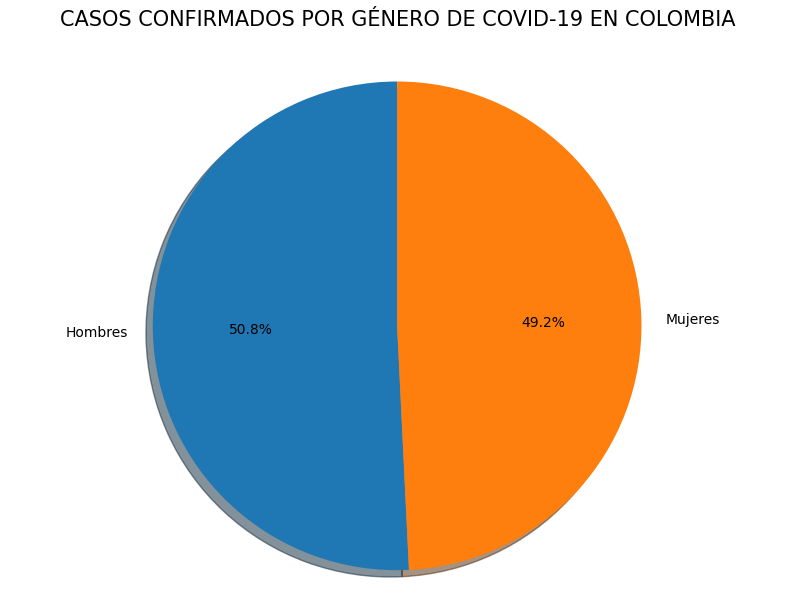
\includegraphics[scale=0.4]{Pictures/GraficoTorta_Genero_Covid_Colombia_30-09-20.png}
    \caption{Gráfico torta por Genero}
    \label{g1}
\end{figure}

La gráfica generada en el Listing \ref{ciu} es la mostrada en la Figura \ref{g2}, exponiendo los datos clasificados por ciudades de los casos de COVID-19.


\begin{figure}[H]
    \centering
    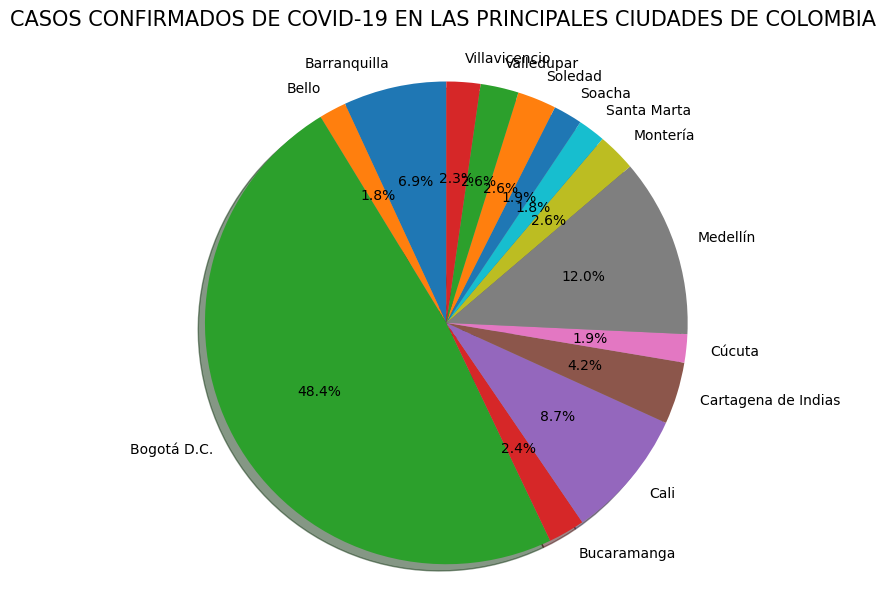
\includegraphics[scale=0.4]{Pictures/GraficoTorta_Casos_Ciudad_Covid_Colombia_30-09-20.png}
    \caption{Gráfico torta por Ciudades}
    \label{g2}
\end{figure}

La gráfica generada en el Listing \ref{edad} es la mostrada en la Figura \ref{g3}, exponiendo los datos clasificados por ciudades de los casos de COVID-19.



\begin{figure}[H]
    \centering
    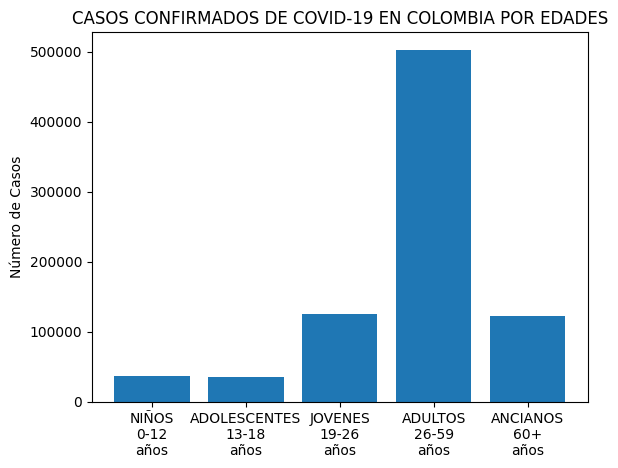
\includegraphics[scale=0.4]{Pictures/GraficoBarras_Edad_Covid_Colombia_30-09-20.png}
    \caption{Gráfico barras por Edades}
    \label{g3}
\end{figure}

La gráfica generada en el Listing \ref{esta} es la mostrada en la Figura \ref{g4}, exponiendo los datos clasificados por ciudades de los casos de COVID-19.



\begin{figure}[H]
    \centering
    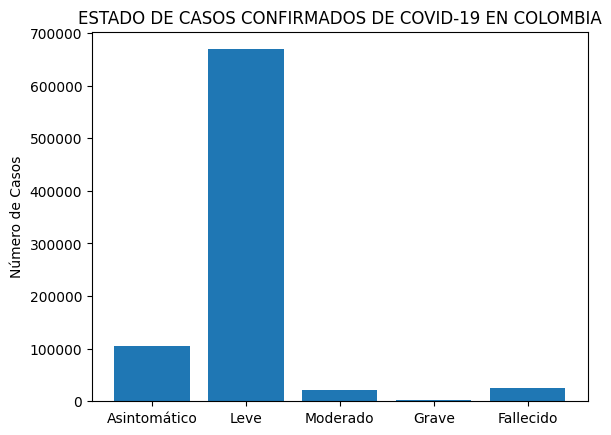
\includegraphics[scale=0.4]{Pictures/GraficoBarras_Estado_Covid_Colombia_30-09-20.png}
    \caption{Gráfico barras por Estado de casos}
    \label{g4}
\end{figure}

\subsection{Resultados Update-2 entrega}\label{sec:re2}

Las gráficas generada a partir del código del Listing \ref{colR2} son mostradas en las figuras \ref{g5}, figura \ref{g6} y figura \ref{g7}

\begin{figure}[H]
    \centering
    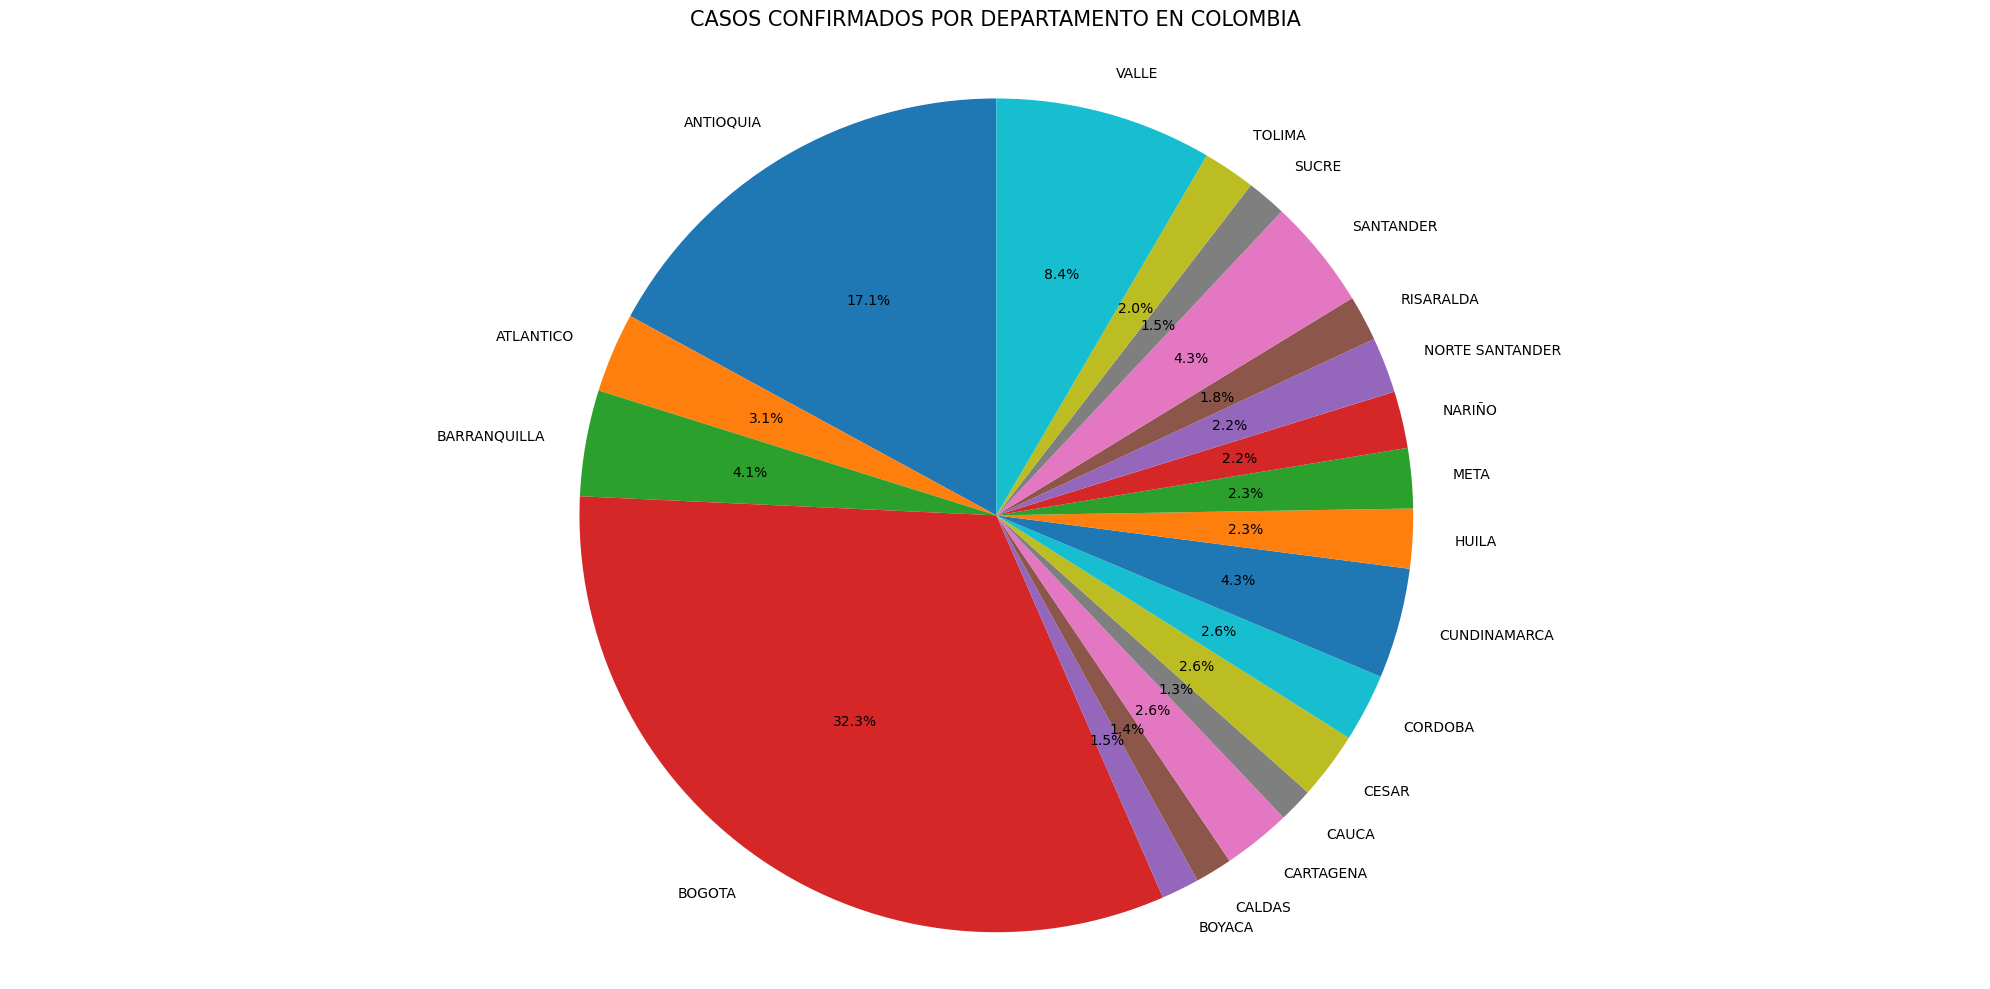
\includegraphics[scale=0.3]{PicturesUpdate/GraficoCircular_Departamento_Covid_Colombia_02-11-20.png}
    \caption{Gráfico de torta-Casos confirmados por departamentos}
    \label{g5}
\end{figure}

\begin{figure}[H]
    \centering
    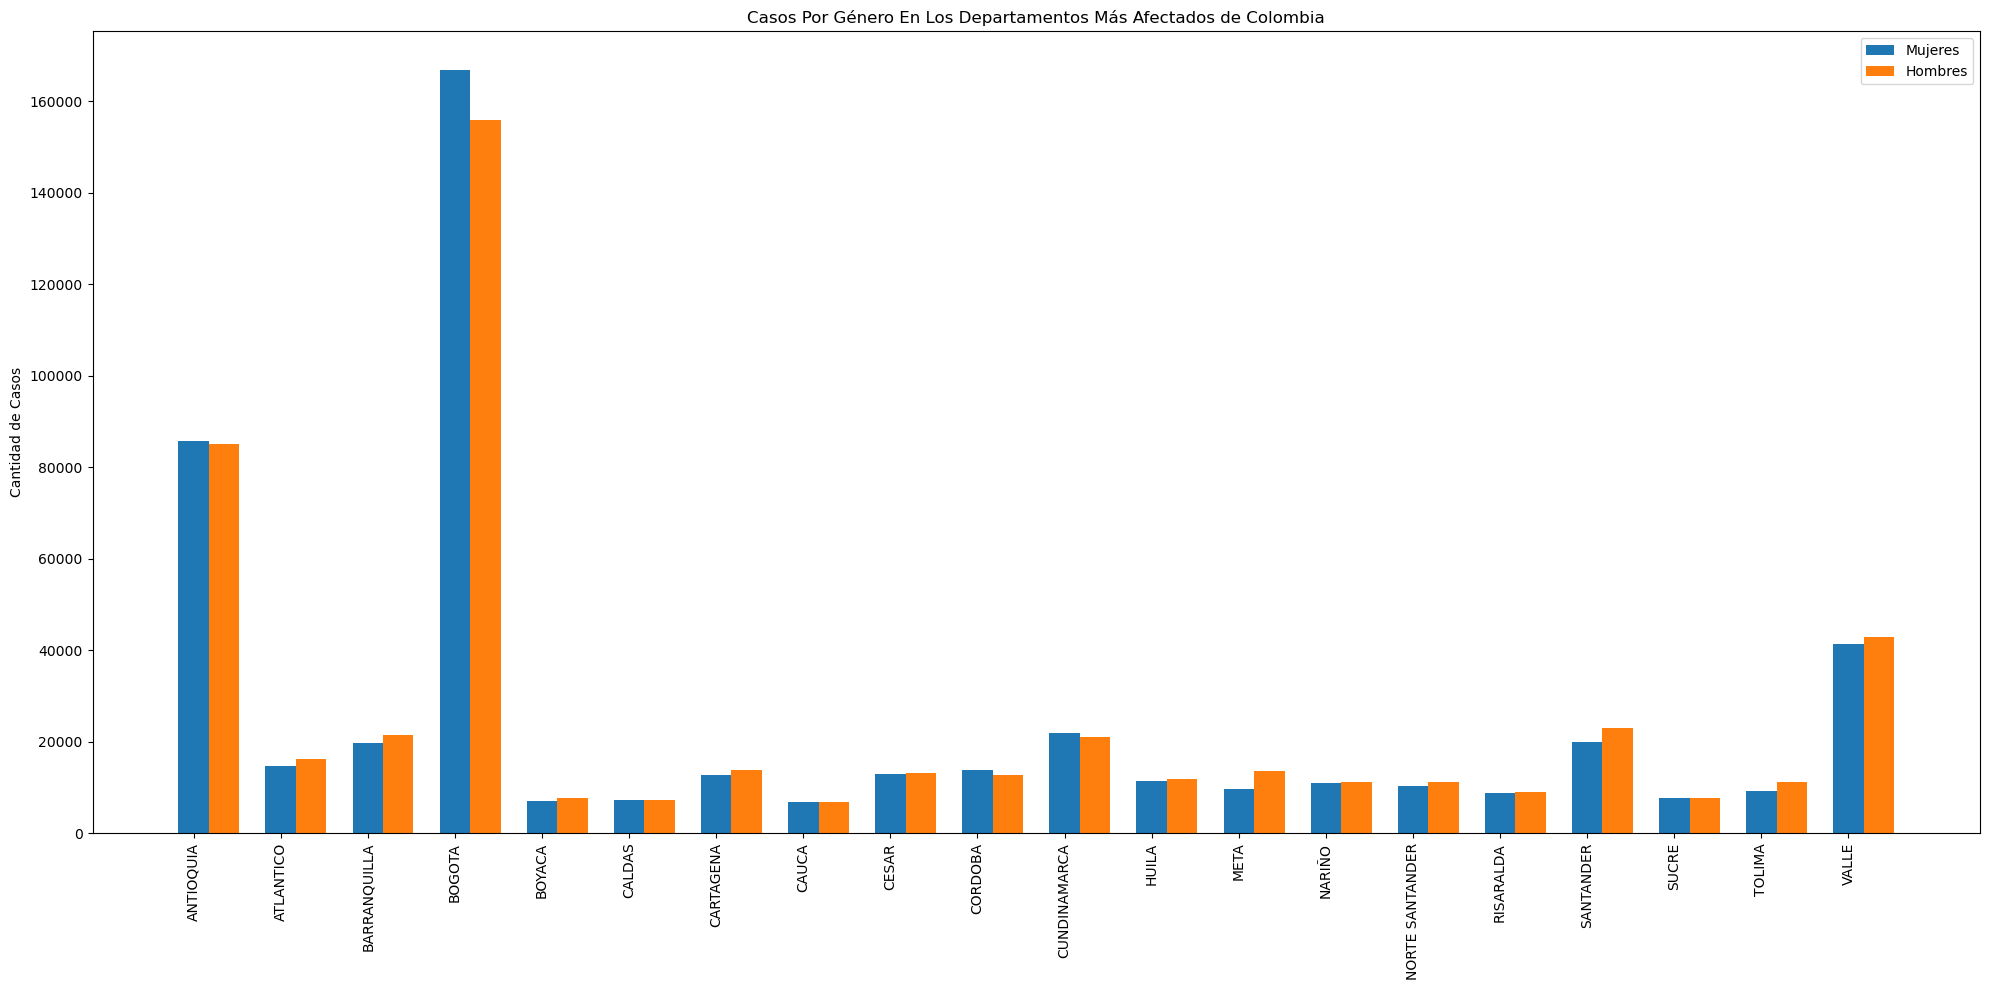
\includegraphics[scale=0.3]{PicturesUpdate/GraficaBarras_Genero_Covid_Departamento_Colombia_02-11-20.png}
    \caption{Gráfico de barras-Casos por genero departamentos mas afectados de Colombia}
    \label{g6}
\end{figure}

\begin{figure}[H]
    \centering
    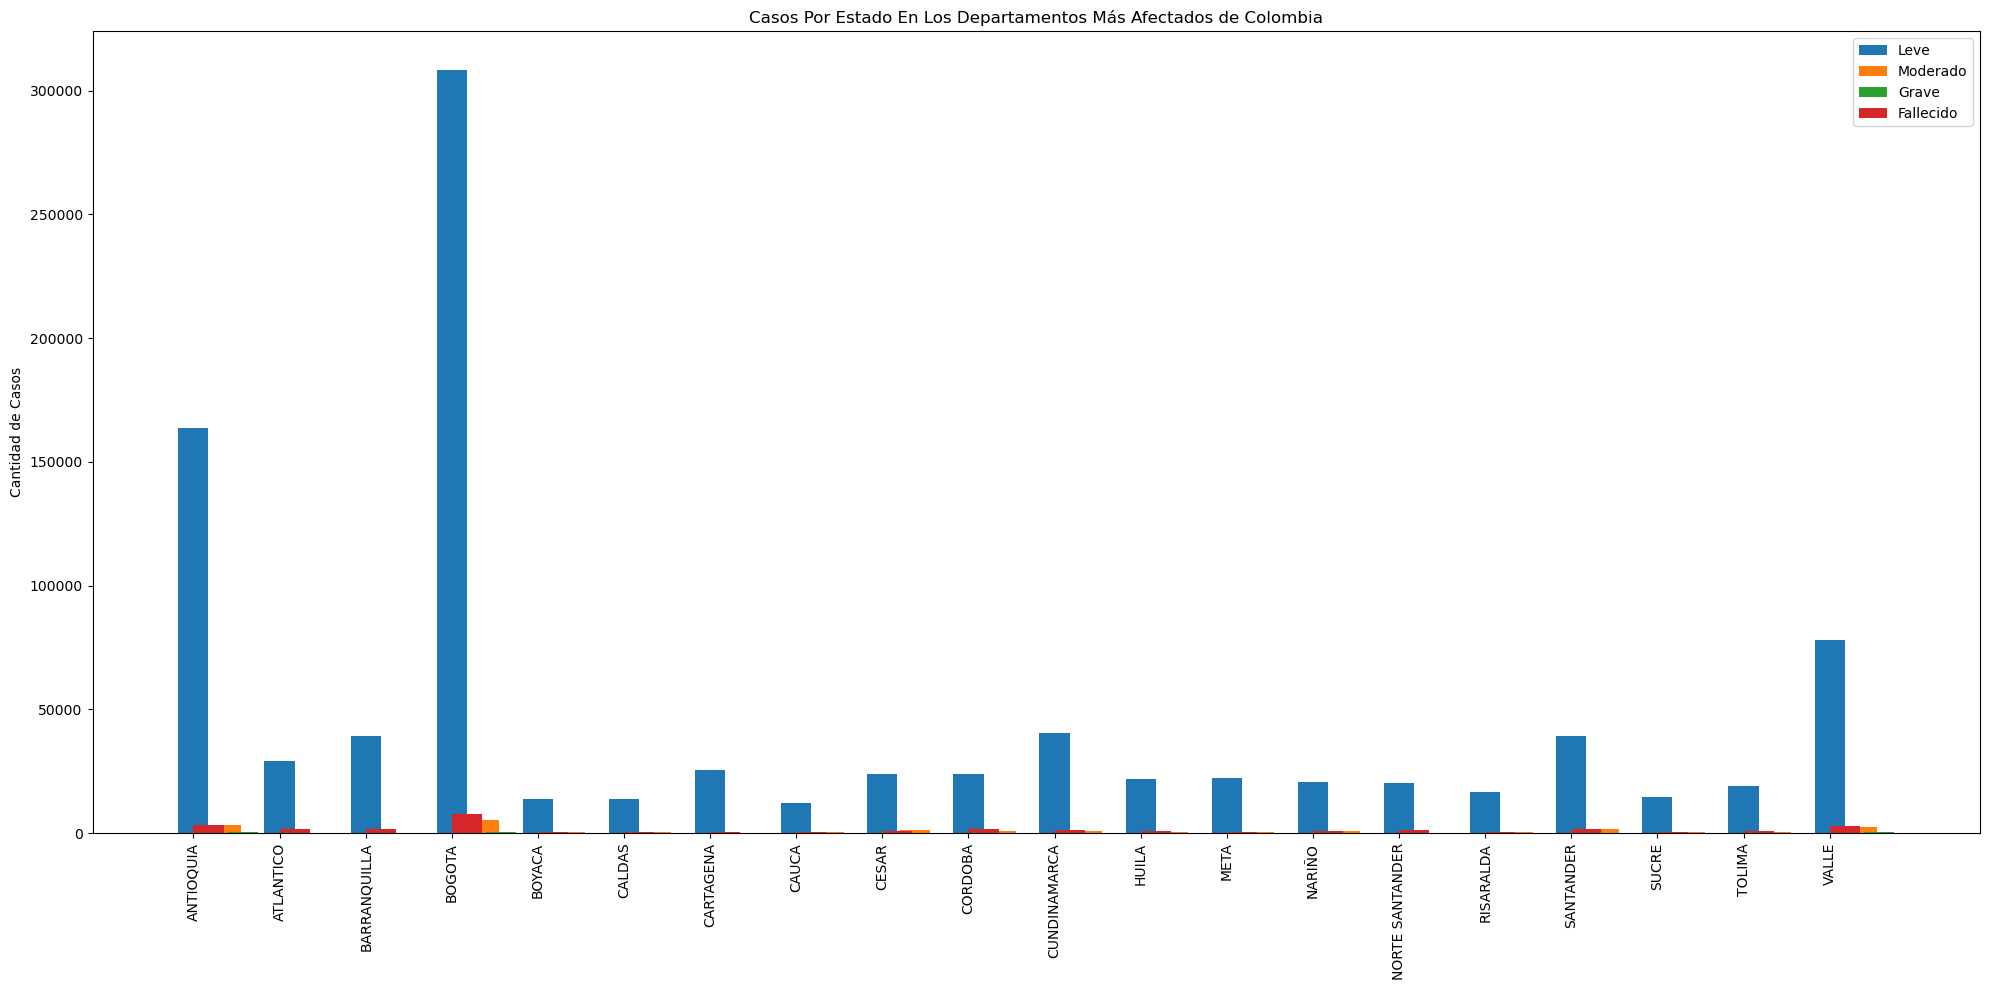
\includegraphics[scale=0.3]{PicturesUpdate/GraficaBarras_Estado_Covid_Departamento_Colombia_02-11-20.png}
    \caption{Gráfico de barras-Casos por estado departamentos mas afectados de Colombia}
    \label{g7}
\end{figure}
\clearpage

Las gráficas generadas a partir del código del archivo BogotaLocalidades.py son mostradas en las figuras \ref{g8}, figuras \ref{g9}, figuras \ref{g10} y figuras \ref{g11}.

\begin{figure}[H]
    \centering
    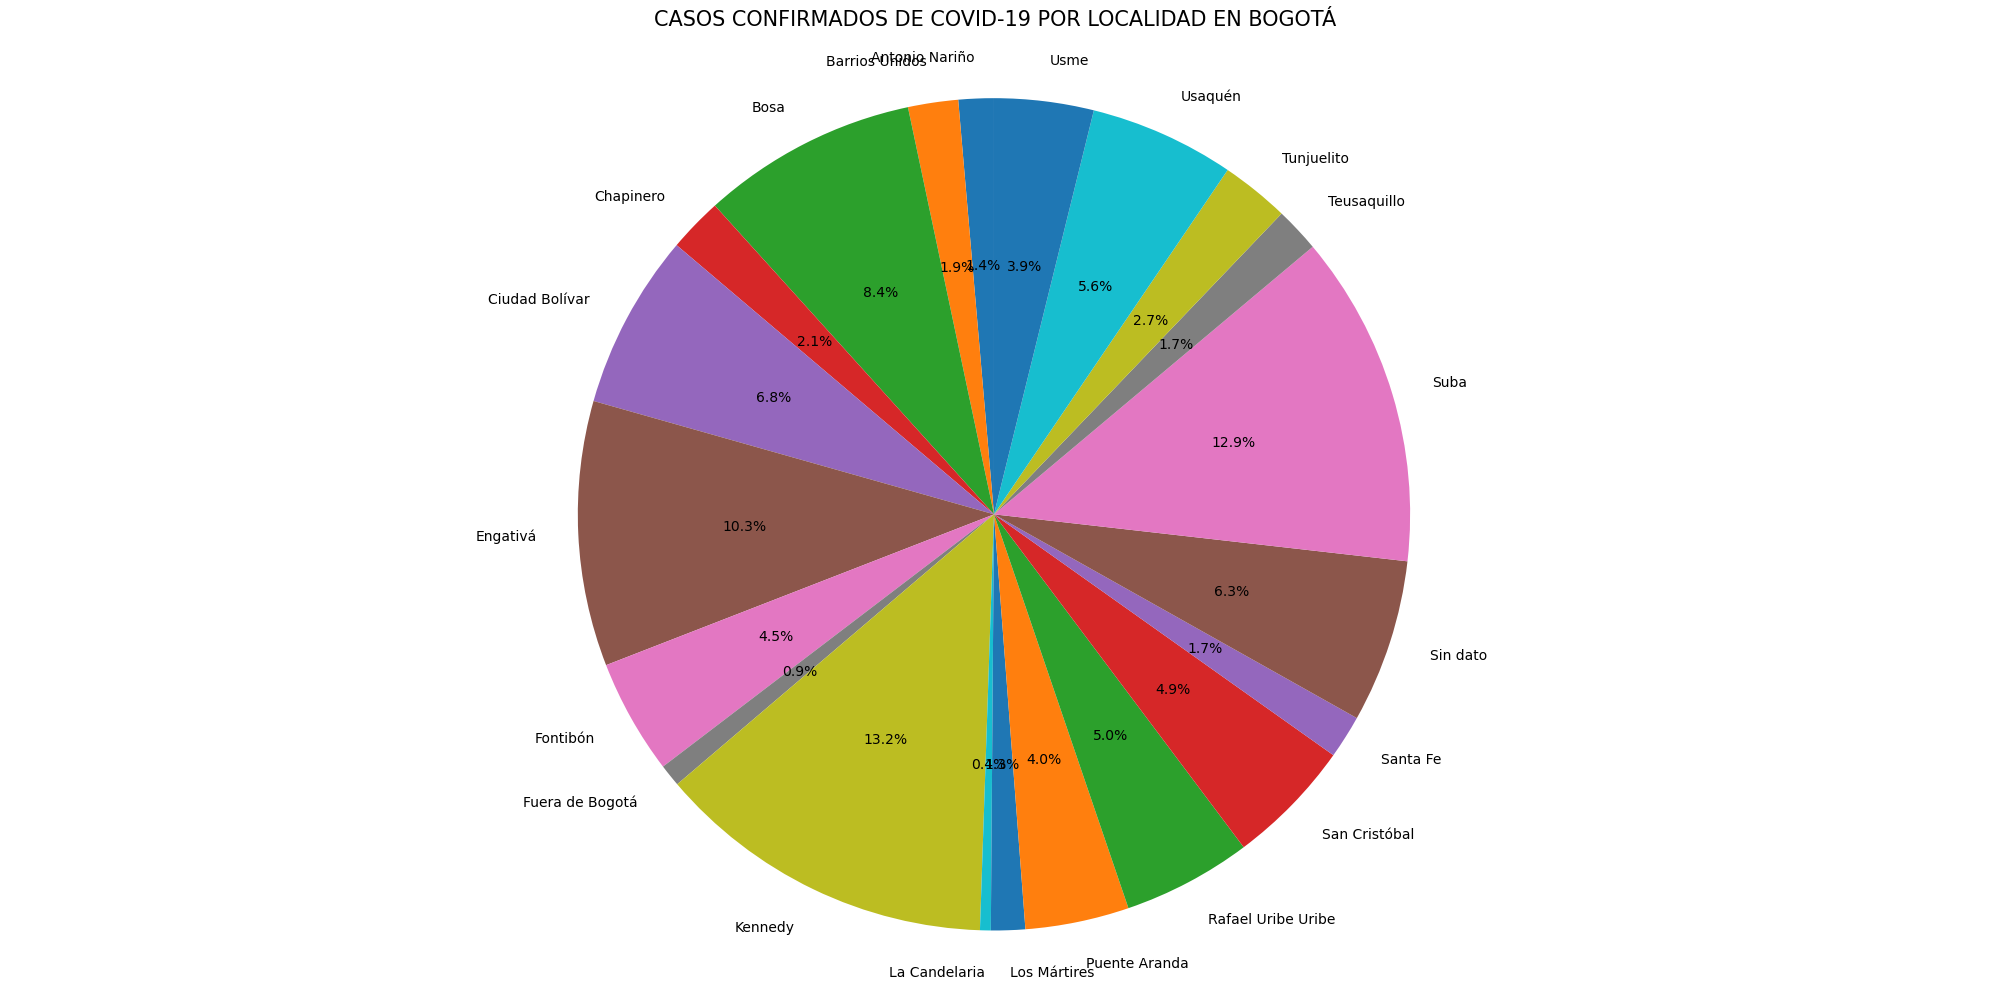
\includegraphics[scale=0.3]{PicturesUpdate/GraficoCircular_Covid_Localidad_Bogota_02-11-20.png}
    \caption{Gráfico de torta-Casos confirmados por localidad en Bogota}
    \label{g8}
\end{figure}


\begin{figure}[H]
    \centering
    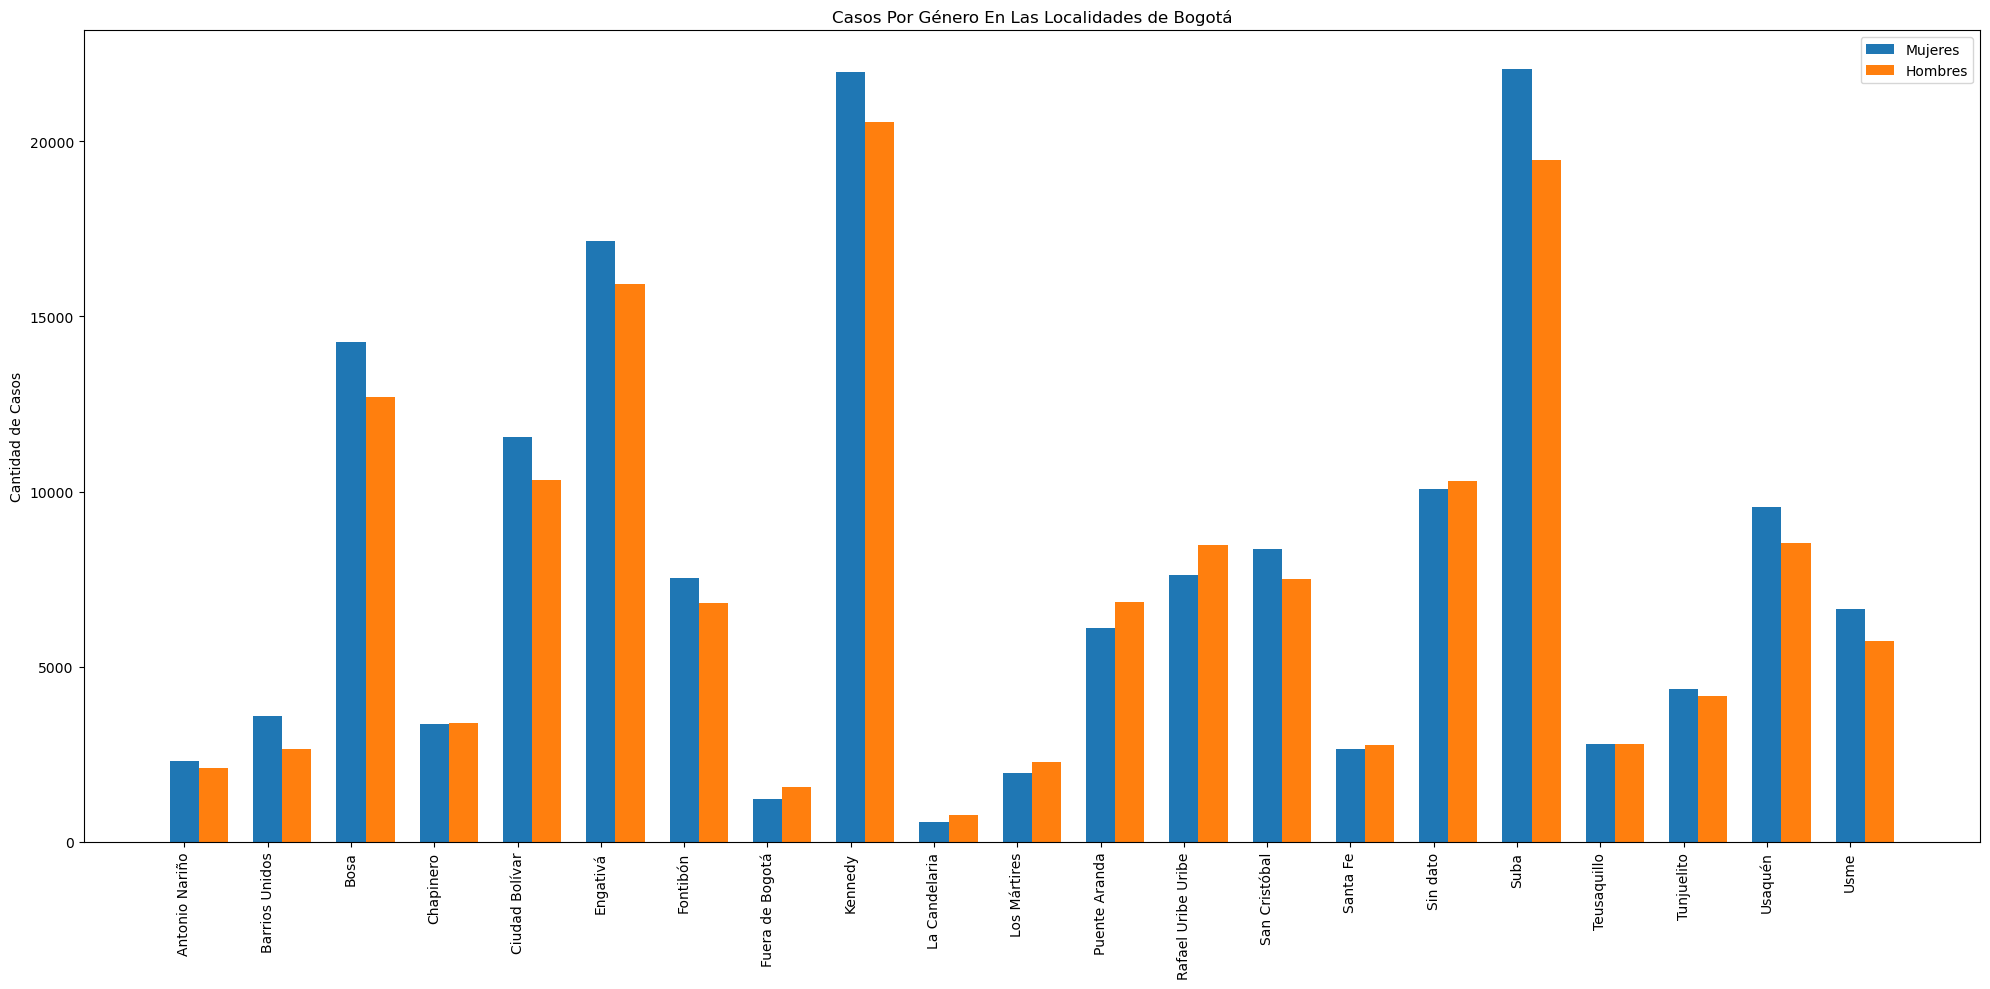
\includegraphics[scale=0.3]{PicturesUpdate/GraficaBarras_Genero_Covid_Localidad_Bogota_02-11-20.png}
    \caption{Gráfico de barra-Casos por genero Localidades Bogota}
    \label{g9}
\end{figure}

\begin{figure}[H]
    \centering
    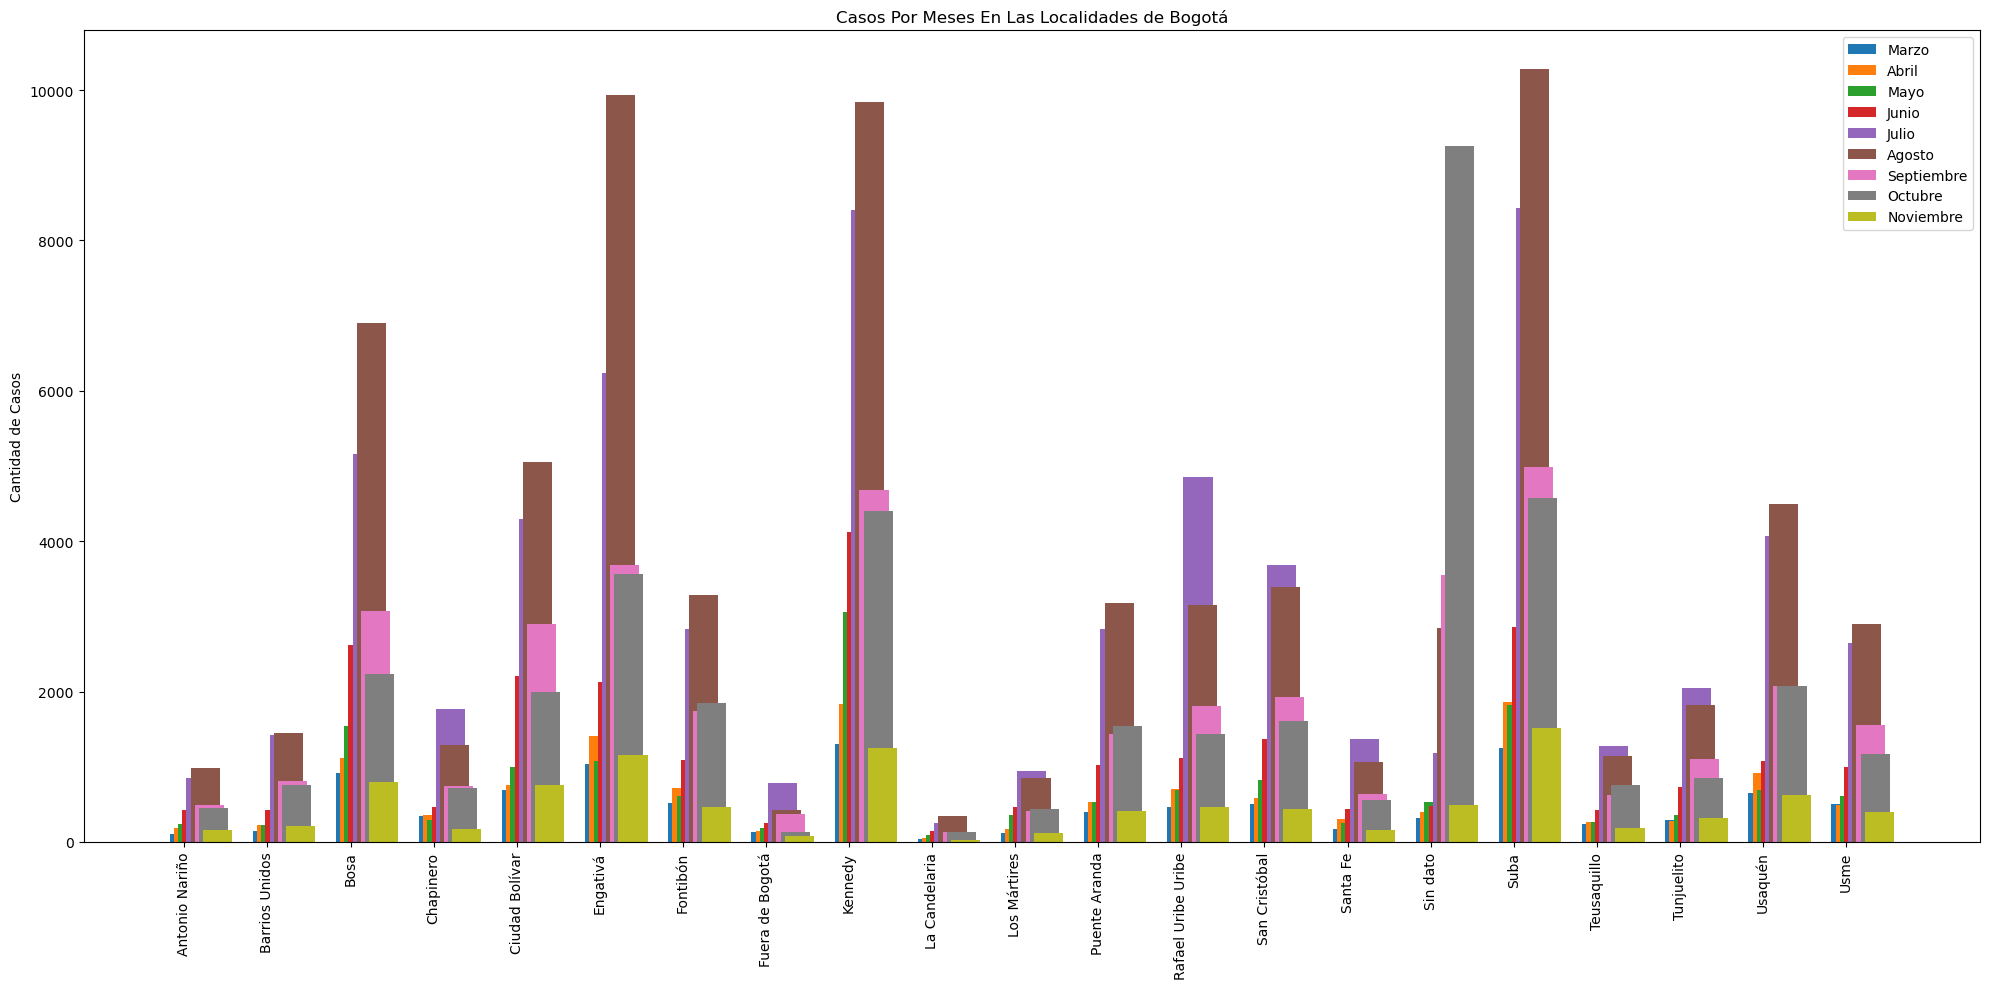
\includegraphics[scale=0.3]{PicturesUpdate/GraficaBarras_Mes_Covid_Localidad_Bogota_02-11-20.png}
    \caption{Gráfico de barra-Casos por meses localidades Bogota}
    \label{g10}
\end{figure}


\begin{figure}[H]
    \centering
    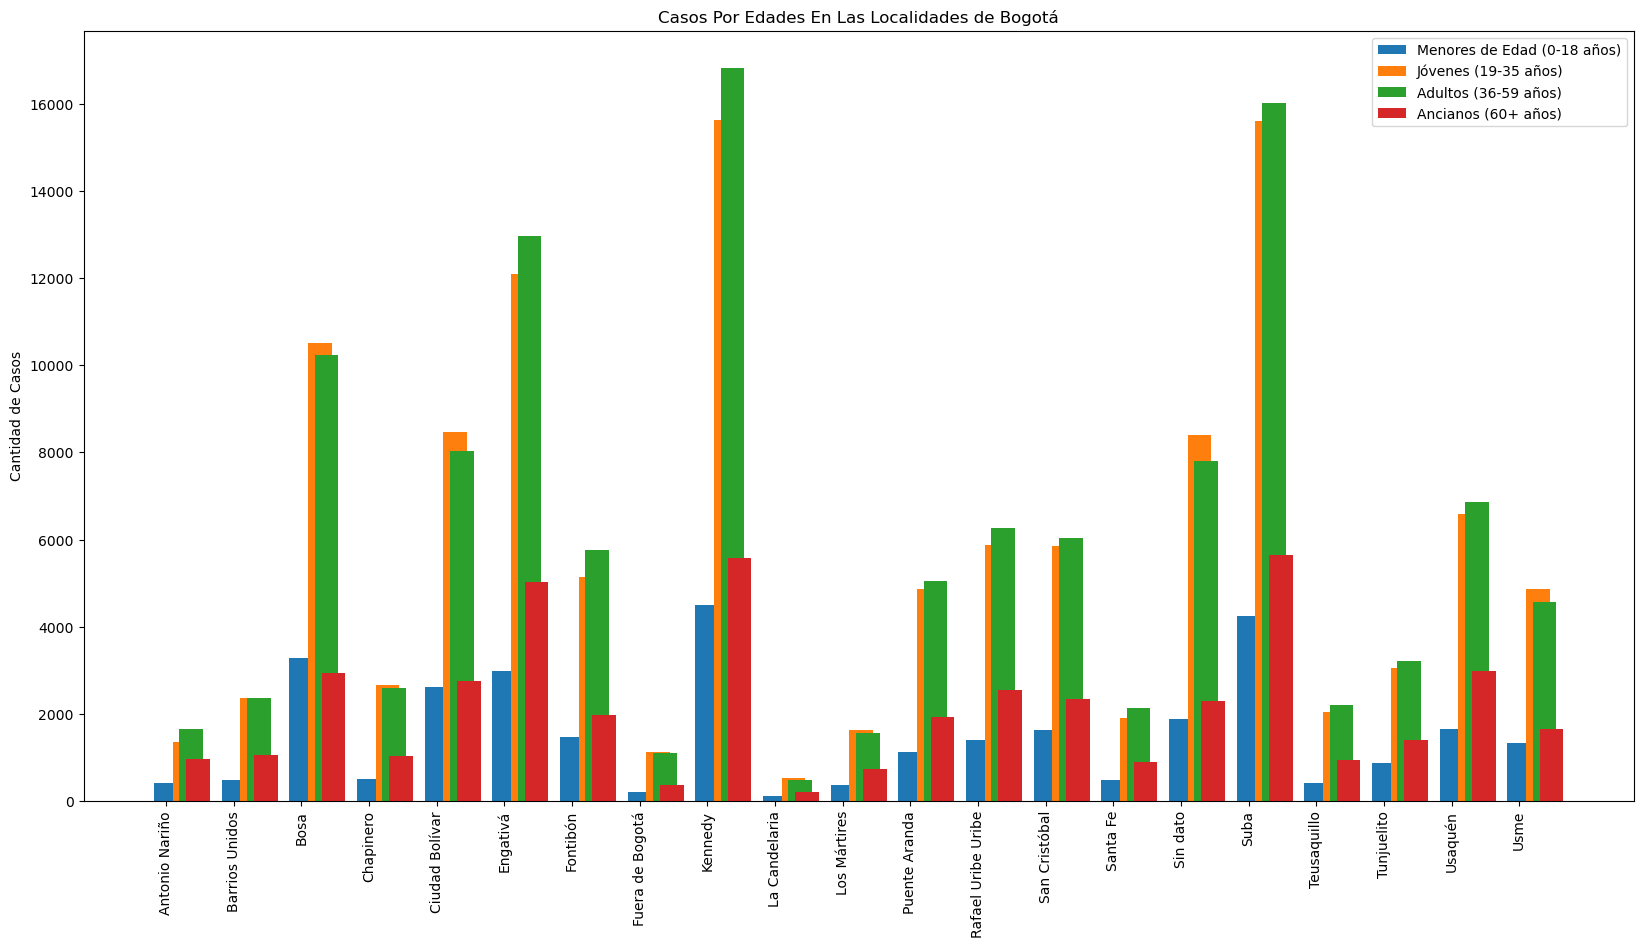
\includegraphics[scale=0.3]{PicturesUpdate/GraficaBarras_Edad_Covid_Bogota_02-11-20.png}
    \caption{Gráfico de barra-Casos por edades en localidades Bogota}
    \label{g11}
\end{figure}
\clearpage
Los mapas de calor expuestos en las figuras \ref{g12} y \ref{g13} fueron de mucha ayuda para poder extraer información y ser usada para el tratamiento de esta. Siendo manejados en los archivos MapaColombia.py y MapaBogota.py con un enlace directo a dichos mapas.

\begin{figure}[H]
    \centering
    \subfigure[Mapa Colombia.]{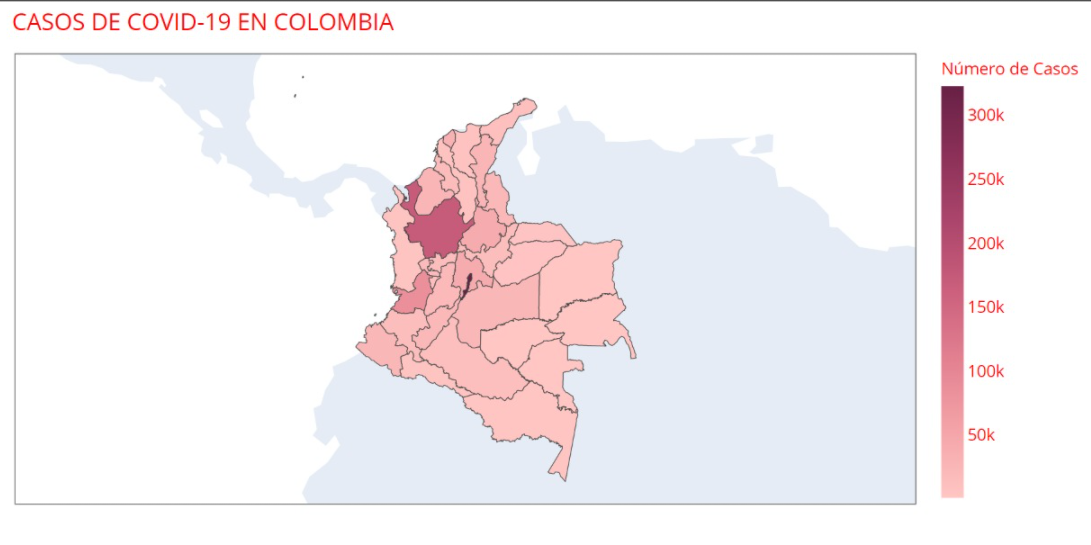
\includegraphics[scale=0.3]{PicturesUpdate/mapa1.PNG}}
    \hspace{2.1mm}
    \subfigure[Mapa Bogota.]{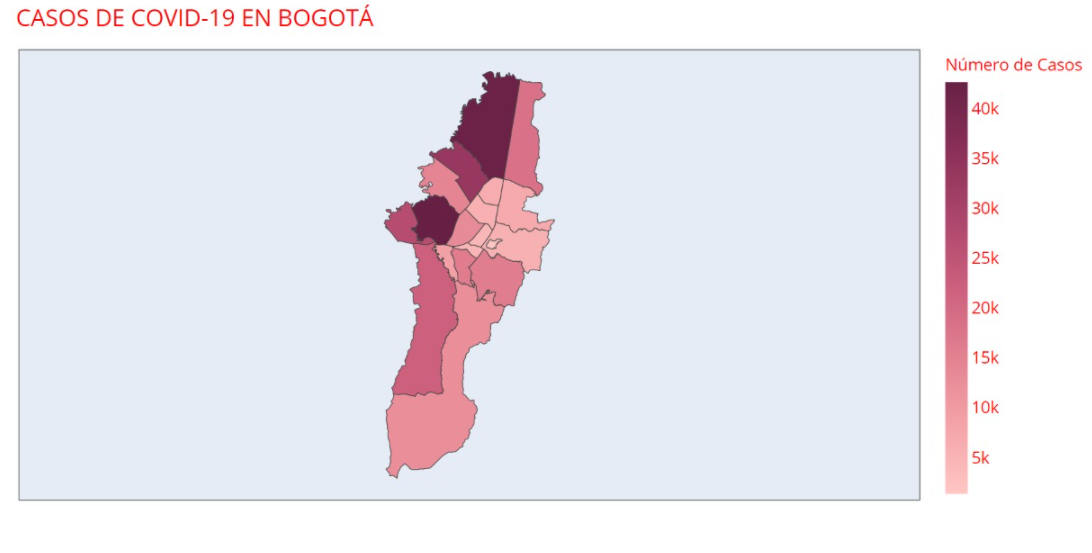
\includegraphics[scale=0.3]{PicturesUpdate/mapa2.PNG}} 
    \caption{Mapas de calor}
    \label{mosaico}
\end{figure}




\section{Conclusiones}
\label{sec:conclusions}
% Escriba su texto aquí
El manejo exitoso del entorno de programación Python, fue exitoso debido a que las gráficas fueron generadas satisfactoriamente, mediante los datos obtenidos de una base de datos en Internet, que expresa datos reales sobre los casos conocidos del COVID-19 en Colombia. Dichos datos fueron recolectados mediante métodos programados y explicados en el entorno Python. 
\nocite{*}
\label{sec:biblio}
\bibliography{bib/biblio}
\bibliographystyle{IEEEtran}



\end{document}


